\documentclass[12pt,a4paper,utf8x]{report}
\usepackage [frenchb]{babel}

%\usepackage{ucs}
\usepackage{graphicx}
\usepackage{caption}
\usepackage[utf8x]{inputenc}
\usepackage{multicol}
\usepackage{url} % Pour avoir de belles url
\usepackage {geometry}
%\usepackage {listings} %Pour mettre du code source 
\usepackage{verbatim}
\usepackage{lscape} % Pour pouvoir passer en paysage
\usepackage{geometry}
\geometry{left=2.5cm,right=2.5cm,vmargin=2cm}

%chapitre---------------------------------------------------------------------
 
%%%% debut macro pour enlever le nom chapitre %%%%
\makeatletter
\def\@makechapterhead#1{%
  \vspace*{50\p@}%
  {\parindent \z@ \raggedright \normalfont
    \interlinepenalty\@M
    \ifnum \c@secnumdepth >\m@ne
        \Huge\bfseries \thechapter\quad
    \fi
    \Huge \bfseries #1\par\nobreak
    \vskip 40\p@
  }}

\def\@makeschapterhead#1{%
  \vspace*{50\p@}%
  {\parindent \z@ \raggedright
    \normalfont
    \interlinepenalty\@M
    \Huge \bfseries  #1\par\nobreak
    \vskip 40\p@
  }}
\makeatother
%%%% fin macro %%%% 


\begin{document}

\begin{titlepage}
\begin{flushright}
   	
\includegraphics[scale=0.30]{univorleans.png}\\ 
   	   	Département Informatique
\end{flushright}
\vspace{30mm}
\begin{center}
\huge{Mémoire intermédiaire \\Travaux d'étude et de recherche }\\
\vspace{8mm}
\large{Sujet : Android au pays des liseuses}\\
\vspace{3mm}
\large{Proposé et encadré par : Ollinger Nicolas}
\vspace{3mm}
\large{\\Réaliser par :}\\
\large{Fontorbe Jordan, Guillaume Arthur, Monediere Tristan, \\Rubagotti Joris}\\
\end{center}
\begin{figure}[b!]
\begin{flushright}
~~\\ ~~\\ ~~\\ ~~\\ ~~\\ ~~\\ ~~\\
\large{Année : 2012-2013}
\end{flushright}
\end{figure}
\end{titlepage}

\tableofcontents
\clearpage

\chapter{Résumé du projet}

Notre projet est proposé par M. OLLINGER et nous entraîne dans le monde des liseuses. Il consiste à étudier dans un premier temps les spécificités du déploiement d'Android sur une liseuse. Dans un second temps, d'émuler la plate-forme à l'aide d'une machine virtuelle sur un écran déporté sur un ordinateur. Tout le développement se concentrera sur la liseuse Sony PRS-T1 et son environnement Android fourni par notre chef de projet. 

%\section{Documentation}
%La première partie du projet a pour objectif de se documenter sur le sujet, c'est à dire la technologie du papier électronique et comment elle est mise en oeuvre au travers des différentes couches matérielles et logicielles.
%Cette partie va servir a la production de ce premier document de synthèse. 
%\section{Écriture du client RFB}
%Cette étape, a pour but de s'approprier les outils mis à notre disposition pour le développement. Il faudra dans un premier temps tester l'image de la liseuse. Puis mettre en oeuvre l'environnement de développement ltib de Freescale pour i.MX508. Il faut ensuite écrire un programme de test du framebuffer eink et ajouter un ioctl de mise à jour pour ensuite développer le support du gadget USB Ethernet au noyau. Il faut aussi ajouter ce module à l'image de test et une connexion via ssh. Il faut modifier DirectFB pour le support e-ink. Il faudra enfin modifier le protocole RFB pour supporter les mises à jour ioctl et mettre en oeuvre un client RFB pour la liseuse après avoir créé un serveur de gestion des mises à jour et effectuer des tests intensifs.
%\section{E-ink sous qemu via VNC}
%L'objectif de cette étape est de comprendre la gestion du framebuffer par l'émulateur qemu pour pouvoir y ajouter la gestion des ioctl. Dans un deuxième temps la compréhension de l'option VNC de qemu permettra l'ajout de l'extension RFB du client de la liseuse. Enfin des tests seront menés pour valider l'étape.
%\section{Liseuse Android sous qemu}
%Dans cette étape la compréhension des versions e-ink d'Android chez Freescale et Sony permettra la mise en place de cette pile dans l'émulateur. Cette étape sera testée à l'aide d'applications Sony. Enfin nous pourront écrire nos propres applications pour l'émulateur.
%\section{Simulateur d'écran E-ink}
%Cette dernière étape a pour objectif d'écrire un simulateur raisonnable d'écran e-ink. Celui-ci devra contenir une option de debug permettant d'afficher les zones de mise à jour. Le simulateur sera ensuite intégré à l'émulateur. Cette étape se terminera par des tests.
\section[Intruduction]{Introduction au domaine}


\subsection[E-Ink]{Technologie E-Ink}
\begin{frame}{Technologie E-Ink}
	%% A compléter par Arthur
\end{frame}


\subsection[Sony PRS-T1]{Liseuse Sony PRS-T1}

\begin{frame}{Caractéristiques principales} %% Liseuse en générale
	\begin{block}{Caractéristiques Sony PRS-T1}
		\begin{itemize}
			\item Processeur iMX508
			\item Écran E-Ink 6 pouces
			\item Résolution jusqu'à 16 niveaux de gris
			\item Interfaces USB
			\item WiFi
			\item Mémoire : 2Go (extensible par microSD)
		\end{itemize}
	\end{block}
\end{frame}

\begin{frame}{Processeur iMX508} %% partie iMX508
	\begin{block}{iMX508}
	\begin{itemize}
		\item{Développé par Freescale}
		\item{Architecture ARM Cortex A8}
		\item{Faible consommation d'énergie}
		\item{Bonnes performances}
		\item{Contrôleur d'écran intégré}
	\end{itemize}
	\end{block}
\end{frame}

\begin{frame}{Modules}
	\begin{block}{EPDC (Electrophoretic Display Controller)}
		\begin{itemize}
			\item{Dirige les signaux (waveform)}
			\item{Mise à jour partielle ou totale}
		\end{itemize}
	\end{block}
	\begin{block}{ePXP (enhanced Pixel Pipeline}
		\begin{itemize}
			\item Transparence
			\item Rotation d'image
			\item Agrandissement / Réduction d'image
		\end{itemize}
	\end{block}
\end{frame}

\begin{frame}{Architecture du processeur iMX508} %% Schéma
	\begin{figure}
		\begin{center}
			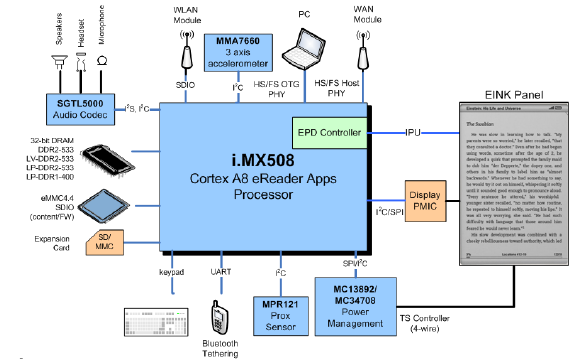
\includegraphics[scale=0.65]{iMX508.png}
		\end{center}
	\end{figure}
\end{frame}

\begin{frame}{Hack de la liseuse}
	\begin{block}{Mise à jour du firmware}
		\begin{itemize}
			\item Nécessite les clés privés de Sony
			\item Accès total à la liseuse
			\item Risque d'endommager la liseuse
		\end{itemize}
	\end{block}
	\begin{block}{Mode Recovery}
		\begin{itemize}
			\item Nécessite la recompilation du noyau
			\item Modifications sans risques
		\end{itemize}
	\end{block}
\end{frame}

\chapter{Analyse de l'existant}
\chapter{Besoins non fonctionnels}
\section{Hacks de la PRS-T1}

La PRS-T1 étant fermé, il nous est impossible dans sa configuration de base de pouvoir y ajouter la mise à jour 
de l'affichage depuis une machine hôte.
Plusieurs méthode existent pour débloquer la liseuse : 

\subsubsection{Mise a jour du firmware}

La méthode la plus répandues pour débloquer la liseuse consiste à faire une mise à jour du firmware.
La liseuse n'acceptant que les mises à jour signée par Sony. Les clefs privées de cette signature étant connues des hackers (elles sont stoquées dans la liseuse pour la vérification).

Plusieurs firmware modifié existe déjà pour mettre à jour la liseuse, c'est derniers débloque complètement la liseuse tout en gardant les logiciels Sony pré-installé.

Cette méthode dispose donc de plusieurs avantages : 
	\begin{itemize}
		\item permet un accès total a la liseuse (installation d'application Android, ...)
		\item on conserve les fonctions normale de la liseuse (logiciel de lecture Sony)
	\end{itemize}
Cependant le fait de modifier le firmware interne de la liseuse comporte certains risques : 
	\begin{itemize}
		\item risque de rendre la liseuse inutilisable
		\item perte de la garantie constructeur
	\end{itemize}

Étant donné que la PRS-T1 est un prêt de M. Ollinger cette méthode de hack comporte trop de risques.

\subsubsection{Utilisation du mode Recovery}

Une autre méthode de hack consiste à utiliser le mode recovery de la liseuse.
Ce mode permet normalement de récupérer la liseuse suite à un problème.
Pour entrer en mode recovery la liseuse a besoin d'un  système de fichier de récupération.
Ce dernier pouvant être situé sur une carte mémoire externe.

Cette méthode réduits les risques encouru lors de la manipulation car un simple redémarrage de la liseuse, 
suffit pour revenir au système de base.

les caractéristiques de cette méthodes sont  : 
%Les avantages de cette méthodes sont : 
\begin{itemize}
	\renewcommand{\labelitemi}{$\bullet$}
	\item Avantages : 
	\begin{itemize}
		\item risque minime pour la liseuse
		\item permet des modifications importante (car on fait nous même le système à partir des sources du noyau fournit par Sony)%un peu long non ?
	\end{itemize}
	\item désavantages : 
		\begin{itemize}
			\item nécessite un pc hôte pour la mise en place du système (nécessitent de compiler le noyau)
			\item On repart de zéro donc on n'a pas accès aux application sony (pour la lecture d'Ebook notamment)
			\item nécessite beaucoup de travail car on repart avec uniquement le noyau.
		\end{itemize}
\end{itemize}
\section{Risque}
\subsection{Les Waveformes}
	Le driver permet de redéfinir les fonctions de waveforme du contrôleur.
Cependant le bon fonctionnement des écrans E-Ink dépend fortement de ces fonctions, modifier ces fonctions peut donc entraîner dans le meilleur des cas une différence entre la représentation virtuelle de l'affichage et ce que va réellement afficher l'écran, dans le pire cas cela peu endommager de manière définitive l'écran de la liseuse.

\section{Tests}

La spécificité des liseuses venant de leur écran il faut faire attention a respecter au maximum le comportement de ce dernier pour faire un environnement de développement dédié aux liseuses.

\subsubsection{Taux de rafraîchissement}

Les écrans E-Ink ayant un taux de rafraîchissement assez bas il devient nécessaire de veiller à ne pas le réduire d'avantage.
Pour cela Il va falloir mettre en place un test comparatif entre le rafraîchissement de la liseuse seule et le rafraîchissement avec un ordinateur hôte via VNC.

\subsubsection{Update bloquante}

De la même manière l'ordinateur hôte ne doit pas se comporter de la meme manière qu'avec un écran classique. En effet il serait très facile pour l'hôte de surcharger complètement l'écran en faisant des mises à jour de l'affichage comme il le ferait avec un écran classique. %a véifier un peu tordu
\chapter{Besoins fonctionnels}

Comme énoncé dans le chapitre 1 de ce document, le but du projet est la réalisation d'un émulateur d'une liseuse avec un écran virtuel fonctionnant comme un écran E-Ink directement sur notre machine ayant pour système d'exploitation Linux. La réalisation de ce projet se découpe en plusieurs parties à réaliser dans un ordre strict afin d'aboutir au résultat final souhaité. Ce plan nous a été proposé par notre encadrant de projet M. OLLINGER. N'ayant pas encore eu le temps de tester les points suivants il se peut que certains des éléments ont été mal interprétés d'où la présence possible d'erreurs. D'autres points peuvent aussi manquer de détails.

\section{Conception d'un client RFB pour la liseuse}

Dans un premier temps il nous faut concevoir un prototype de client permettant de mettre à jour l'écran de la liseuse de test via notre ordinateur.

\subsection{DirectFB}
Pour réaliser cela, il nous a été proposé de travailler avec DirectFB. C'est une bibliothèque libre qui fournit à la fois un accès aux composants matériels graphiques (accélération graphique) ainsi qu'aux périphériques d'entrées, et un systèmes de gestion de fenêtres intégrées avec support de la transparence et de calques multiples. Tout ceci à travers l'interface framebuffer de Linux. Nous devons ajouter la gestion des écrans E-Ink dans DirectFB. 
 
\subsection{Client RFB}
Lorsque DirectFB est prêt à être employé, on travaille ensuite sur le protocole RFB (Remote FrameBuffer) qui est un simple protocole permettant des accès à distance à des interfaces graphiques d'utilisateur. On doit ajouter la gestion des mises à jour de l'affichage pour les écrans de type E-Ink via ioctl. De tous ces éléments, on peut ainsi concevoir un client RFB interagissant sur la liseuse et la conception d'un serveur gérant les mises à jour.
\\Les tests consisteront à essayer de produire des changements d'affichage sur la liseuse grâce à des demandes précises envoyées via l'ordinateur de test et transmis par le serveur de mise à jour. 

\newpage

\section{E-Ink QEMU via VNC}

Dans un second temps, on développe la base de l'émulateur, c'est à dire la mise en place d'une machine virtuelle pouvant reproduire les actions nécessaires au fonctionnement d'un écran E-Ink. Pour réaliser cela, nous travaillons sur QEMU qui permet l'émulation de processeur et de machine virtuelle permettant l'exécution de système d'exploitation. On ajoute la gestion des ioctl à QEMU. Ensuite il faut ajouter à l'option VNC de QEMU l'extension RFB du client de la liseuse.
\\Le test consiste à vérifier si depuis une machine virtuelle QEMU utilisant l'image du noyau Linux de la liseuse de test, on peut via VNC interagir avec la liseuse. 


\section{Liseuse Android sous QEMU}

Après la création de la base de l'émulateur, on intègre à celui-ci un système d'exploitation Android conçu pour fonctionner sur une liseuse. Dans notre cas ça sera la version d'Android présente sur notre liseuse de test SONY PRS-T1.
Pour les tests, on lance l'émulateur muni d'Android et on test le fonctionnement des applications SONY fournies de base avec le système d'exploitation.

\section{Simulation d'écran E-Ink}

Pour finir le développement de l'émulateur, on développe un simulateur d'écran E-Ink reproduisant virtuellement le comportement de celui-ci en y ajoutant des fonctionnalités facilitant les tests telles que choisir une zone précise à mettre à jour sur un écran (utile au debug). Ensuite on intègre celui-ci dans notre émulateur.
\\Les tests consisteraient à réaliser des mini-applications, les lancer sur l'émulateur et vérifier les réactions de notre écran virtuel.


\chapter{Résultats de tests}
\begin{landscape}
\chapter{Planning}

\begin{figure}[h!]
\begin{center}

\begin{ganttchart}[y unit title=0.4cm,
y unit chart=0.5cm,
vgrid,hgrid, 
title label anchor/.style={below=-1.6ex},
title left shift=.05,
title right shift=-.05,
title height=1,
bar/.style={fill=gray!50},
incomplete/.style={fill=cyan},
progress label text={},
bar height=0.7,
group right shift=0,
group top shift=.6,
group height=.3,
group peaks={}{}{.2}]{32}
%labels
\gantttitle{Planning}{32} \\
\gantttitle{Février}{8} 
\gantttitle{Mars}{8} 
\gantttitle{Avril}{8} 
\gantttitle{Mai}{8} \\
%tasks
\ganttbar[bar/.style={fill=green, rounded corners=3pt}]{Recherche Doc}{1}{8} \\
\ganttbar[bar/.style={fill=blue, rounded corners=3pt}]{Réunion}{9}{10} \\
\ganttbar[progress=90,bar/.style={fill=orange, rounded corners=3pt}]{Dev DirectFB}{11}{17} \\
\ganttbar[progress=90,bar/.style={fill=orange, rounded corners=3pt}]{Dev Client RFB}{11}{17} \\
\ganttbar[progress=90,bar/.style={fill=orange, rounded corners=3pt}]{Dev Serveur Update}{11}{17} \\
\ganttbar[progress=90,bar/.style={fill=orange, rounded corners=3pt}]{Dev QEMU et VNC}{17}{21} \\
\ganttbar[progress=90,bar/.style={fill=orange, rounded corners=3pt}]{Dev QEMU Liseuse SONY}{18}{22} \\
\ganttbar[progress=90,bar/.style={fill=orange, rounded corners=3pt}]{Dev Simulation Ecran}{23}{27} \\
\ganttbar[bar/.style={fill=yellow, rounded corners=3pt}]{Finalisation}{28}{31}
\end{ganttchart}
\vspace{-0.5cm}
\end{center}
\hspace{7.3cm} \noindent \begin{tabular}{l}
	 \rowcolor{green} \\  
\end{tabular}
Recherche documentaire

\hspace{7.3cm} \noindent \begin{tabular}{l}
     \rowcolor{blue} \\  
\end{tabular}
Réunion du groupe pour mettre en commun tous les éléments et répartir les taches 

\hspace{7.3cm} \noindent \begin{tabular}{l}
     \rowcolor{orange} \\  
\end{tabular}
Phase de développement

\hspace{7.3cm} \noindent \begin{tabular}{l}
     \rowcolor{cyan} \\  
\end{tabular}
Phase de test

\hspace{7.3cm} \noindent \begin{tabular}{l}
     \rowcolor{yellow} \\  
\end{tabular}
Finalisation du TER \\
\caption{Planning de réalisation du projet}
\end{figure}
\end{landscape}
\chapter{Bibliographie}

\end{document} 